\documentclass[aspectratio=169,10pt]{beamer}

% Prefer the modern Metropolis theme when it is installed. Otherwise, fall back
% to the stock Beamer theme so this template still compiles on a minimal setup.
\IfFileExists{beamerthememetropolis.sty}{%
  \usetheme[progressbar=frametitle,numbering=fraction]{metropolis}
  \metroset{block=fill}
}{%
  \usetheme{Madrid}
  \usecolortheme{dolphin}
  \setbeamertemplate{navigation symbols}{}
}

\usepackage{amsmath}
\usepackage{array}
\usepackage{booktabs}
\usepackage{graphicx}
\usepackage{siunitx}

\graphicspath{{figures/}{../saltmix-manuscript/figures/}{../saltmix-manuscript/figures-SI/}}

\definecolor{SaltBlue}{HTML}{1B4D89}
\definecolor{SaltTeal}{HTML}{1F9E89}
\definecolor{SaltOrange}{HTML}{D96C2C}
\definecolor{SaltInk}{HTML}{243142}

\setbeamercolor{normal text}{fg=SaltInk}
\setbeamercolor{frametitle}{fg=white}
\setbeamercolor{title}{fg=SaltBlue}
\setbeamercolor{progress bar}{fg=SaltTeal,bg=SaltBlue!18}
\setbeamercolor{alerted text}{fg=SaltOrange}
\setbeamercolor{block title}{fg=white,bg=SaltBlue}
\setbeamercolor{block body}{fg=SaltInk,bg=SaltBlue!6}

\setbeamertemplate{itemize item}{\color{SaltTeal}$\blacktriangleright$}
\setbeamertemplate{itemize subitem}{\color{SaltOrange}$\bullet$}

\newcolumntype{L}[1]{>{\raggedright\arraybackslash}p{#1}}
\newcommand{\best}[1]{\textcolor{SaltTeal}{\textbf{#1}}}
\newcommand{\watchout}[1]{\textcolor{SaltOrange}{\textbf{#1}}}
\newcommand{\slidecaption}[1]{\vspace{0.10cm}{\scriptsize\textbf{#1}}\par}
\newcommand{\figmissing}[1]{%
  \fbox{\parbox[c][0.50\textheight][c]{0.95\linewidth}{\centering #1}}%
}

\title[SaltMix]{Physics-Inspired Neural Models for\\Mixture-Order Extrapolation of Molten Salt Properties}
\subtitle{Component-encoded models for thermophysical and transport properties}
\author[Liang et al.]{Wenshuo Liang, Yuan Yin, Wentao Zhou, Dezhong Wang}
\institute{Shanghai Jiao Tong University\\Shanghai Smartlogic Technology Ltd.}
\date{\today}

\begin{document}

\begin{frame}[plain,noframenumbering]
  \vspace*{0.7cm}
  {\usebeamerfont{title}\usebeamercolor[fg]{title}\inserttitle\par}
  \vspace{0.30cm}
  {\usebeamerfont{subtitle}\usebeamercolor[fg]{subtitle}\insertsubtitle\par}
  \vfill
  {\usebeamerfont{author}\insertauthor\par}
  \vspace{0.10cm}
  {\usebeamerfont{institute}\insertinstitute\par}
  \vspace{0.30cm}
  {\usebeamerfont{date}\insertdate\par}
\end{frame}

\begin{frame}{Question}
  \begin{columns}[T,onlytextwidth]
    \begin{column}{0.55\textwidth}
      \IfFileExists{../saltmix-manuscript/figures/toc_graphic.png}{%
        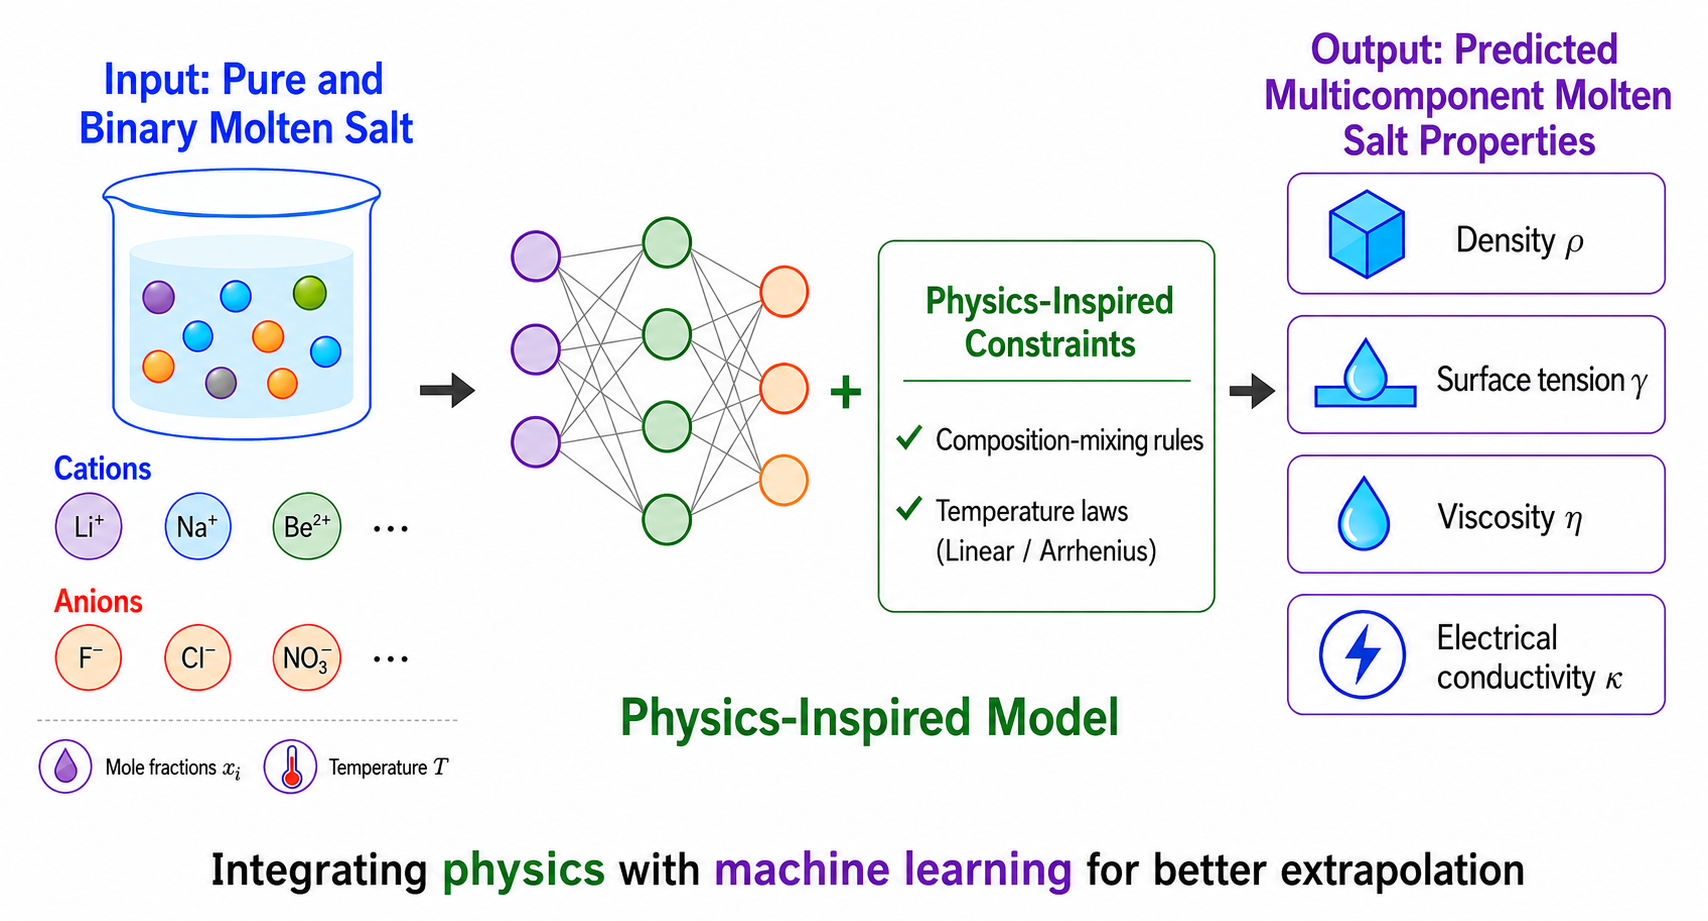
\includegraphics[width=\linewidth]{toc_graphic.png}
      }{%
        \figmissing{TOC graphic}
      }
      \slidecaption{Figure 1: SaltMix graphical overview.}
    \end{column}
    \begin{column}{0.40\textwidth}
      \begin{block}{Question}
        Can models trained on pure and binary salts extrapolate to ternary and higher-order mixtures?
      \end{block}
      \begin{block}{Answer}
        Yes, but the useful physics-inspired constraint is \best{property dependent}.
      \end{block}
    \end{column}
  \end{columns}
\end{frame}

\begin{frame}{Talk Roadmap}
  \tableofcontents
\end{frame}

\section{Motivation}

\begin{frame}{Why This Problem Matters}
  \begin{columns}[T,onlytextwidth]
    \begin{column}{0.56\textwidth}
      \begin{itemize}
        \item Molten salts support nuclear energy, concentrated solar thermal storage, high-temperature electrochemistry, and metallurgy.
        \item Engineering design needs density, viscosity, surface tension, and electrical conductivity across composition and temperature.
        \item Measurements are costly because of high temperature, corrosion, volatility, impurity sensitivity, and container compatibility.
      \end{itemize}
    \end{column}
    \begin{column}{0.38\textwidth}
      \begin{block}{Data bottleneck}
        Low-order systems are relatively well represented; ternary and higher-order mixtures are systematically sparse.
      \end{block}
      \begin{block}{Modeling bottleneck}
        A single mixing rule or temperature law may not fit all target properties.
      \end{block}
    \end{column}
  \end{columns}
\end{frame}

\begin{frame}{Mixture-Order Extrapolation}
  \begin{columns}[T,onlytextwidth]
    \begin{column}{0.48\textwidth}
      \begin{block}{Training domain}
        Pure and binary systems are split into train and validation sets.
      \end{block}
      \begin{block}{Test domain}
        Ternary and higher-order systems are held out.
      \end{block}
    \end{column}
    \begin{column}{0.47\textwidth}
      \begin{itemize}
        \item The task is not complete leave-component-out extrapolation.
        \item The model must recombine learned component, pair, and temperature information.
        \item This matches practical screening, where high-order measurements are scarce.
      \end{itemize}
    \end{column}
  \end{columns}
  \vfill
  \[
    \{\mathrm{pure},\mathrm{binary}\}\longrightarrow
    \{\mathrm{ternary},\mathrm{quaternary},\ldots\}
  \]
\end{frame}

\section{Data and Models}

\begin{frame}{Dataset Construction}
  \begin{columns}[T,onlytextwidth]
	    \begin{column}{0.50\textwidth}
	      \small
	      \begin{itemize}
	        \item Sources: Janz molten salt compilation and MSTDB-TP v4.0.
	        \item Retained inorganic halides and common oxyanion salts; excluded organics, oxides, and sulfides.
	        \item Data were first organized as record-level entries.
	      \end{itemize}
	    \end{column}
    \begin{column}{0.46\textwidth}
      \footnotesize
      \slidecaption{Table 1: Dataset size after sample expansion.}
      \begin{tabular}{lrr}
        \toprule
        Property & Records & Samples \\
        \midrule
        Density & 3,780 & 18,808 \\
        Viscosity & 1,469 & 7,154 \\
        Surface tension & 1,447 & 7,155 \\
        Electrical conductivity & 3,476 & 17,012 \\
        \bottomrule
      \end{tabular}

      \vspace{0.4cm}
      Units: \si{g.cm^{-3}}, \si{mPa.s}, \si{mN.m^{-1}}, and \si{S.cm^{-1}}.
	    \end{column}
	  \end{columns}
	  \vspace{0.20cm}
	  \small
	  \begin{itemize}
	    \item Record-level split: pure/binary records were split 80:20 into train/validation; ternary and higher-order records were held out as test.
	    \item Records were expanded into samples by sampling temperature or composition intervals.
	  \end{itemize}
\end{frame}

\begin{frame}{Component-Encoded Framework}
  \begin{columns}[T,onlytextwidth]
    \begin{column}{0.58\textwidth}
      \IfFileExists{../saltmix-manuscript/figures/SaltMix_mechanism.png}{%
        \includegraphics[width=0.98\linewidth]{SaltMix_mechanism.png}
      }{%
        \figmissing{SaltMix mechanism figure}
      }
      \slidecaption{Figure 2: Component-encoded SaltMix workflow.}
    \end{column}
    \begin{column}{0.38\textwidth}
      \begin{itemize}
        \item Each salt component is encoded by formula, cation, anion, and stoichiometry tokens.
        \item A shared Transformer encoder produces component representations.
        \item Mole fraction and temperature are fused with component features.
        \item Predictor heads impose different physical biases.
      \end{itemize}
    \end{column}
  \end{columns}
\end{frame}

\begin{frame}{Training Details}
  \begin{itemize}
    \item Shared component encoder: 128-dimensional embeddings, two-layer Transformer, four attention heads.
    \item Component latent representation: formula/cation/anion/stoichiometry features fused with mole fraction and normalized temperature.
    \item Optimizer: AdamW, learning rate $5\times10^{-4}$, weight decay $10^{-4}$, batch size 64.
    \item Early stopping patience: 20 epochs; maximum epochs: 200.
    \item Each setting is trained with five random seeds; reported metrics are mean $\pm$ SD.
  \end{itemize}
\end{frame}

\begin{frame}{Three Model Families}
  \begin{block}{Unconstrained}
    \begin{columns}[c,onlytextwidth]
      \begin{column}{0.39\textwidth}
        \footnotesize Set pooling over component representations, followed by direct property prediction.
      \end{column}
      \begin{column}{0.56\textwidth}
        \[
          z=f_\theta(\{s_i,x_i,T\})
        \]
      \end{column}
    \end{columns}
  \end{block}
  \vspace{-0.10cm}
  \begin{block}{CW/CW+RK}
    \begin{columns}[c,onlytextwidth]
      \begin{column}{0.34\textwidth}
        \footnotesize Composition-weighted component terms plus pairwise RK-style corrections.
      \end{column}
      \begin{column}{0.61\textwidth}
        \scriptsize
        \[
          \begin{aligned}
            z_{\mathrm{mix}}
            &= \sum_{i=1}^{C}x_i z_i \\
            &\quad+\sum_{i<j}x_i x_j
            \sum_{k=0}^{N}B^k_{\mathrm{RK},i,j}(x_i-x_j)^k
          \end{aligned}
        \]
      \end{column}
    \end{columns}
  \end{block}
  \vspace{-0.10cm}
  \begin{block}{Temperature constrained}
    \begin{columns}[c,onlytextwidth]
      \begin{column}{0.39\textwidth}
        \footnotesize Linear output for density/surface tension; Arrhenius output for transport properties.
      \end{column}
      \begin{column}{0.56\textwidth}
        \[
          z=a+bT
          \quad \mathrm{or} \quad
          \ln z=\ln a+\frac{b}{T}
        \]
      \end{column}
    \end{columns}
  \end{block}
  \vspace{-0.06cm}
  \begin{center}
    \small \watchout{Hypothesis:} the best inductive bias should match\\
    the target property's dominant physics.
  \end{center}
\end{frame}

\section{Results}

\begin{frame}{Low-Order Held-Out Validation}
  \begin{columns}[T,onlytextwidth]
    \begin{column}{0.49\textwidth}
      \begin{block}{What validation measures}
        Held-out records from pure and binary systems, used for early stopping and model selection.
      \end{block}
      \begin{block}{Why it matters}
        It checks whether each architecture learns the low-order composition--temperature relationships before extrapolation.
      \end{block}
    \end{column}
    \begin{column}{0.47\textwidth}
      \scriptsize
      \setlength{\tabcolsep}{3pt}
      \slidecaption{Table 2: Best low-order validation model by property.}
      \begin{tabular}{L{0.34\linewidth}L{0.32\linewidth}L{0.22\linewidth}}
        \toprule
        Property & Best validation model & Val $r$ \\
        \midrule
        Density & Unconstrained & $0.99\pm0.01$ \\
        Surface tension & Linear & $0.96\pm0.04$ \\
        Viscosity & Unconstrained & $0.99\pm0.00$ \\
        Conductivity & Unconstrained & $0.97\pm0.01$ \\
        \bottomrule
      \end{tabular}

      \vspace{0.35cm}
      \small
      \watchout{Important:} validation ranking does not always predict ternary-and-higher test ranking.
    \end{column}
  \end{columns}
\end{frame}

\begin{frame}{Mixture-Order Extrapolation}
  \scriptsize
  \setlength{\tabcolsep}{3pt}
  \slidecaption{Table 3: Best high-order test model by property.}
  \begin{tabular}{L{0.21\linewidth}L{0.26\linewidth}L{0.15\linewidth}L{0.28\linewidth}}
    \toprule
    Property & Best test model & Test $r$ & Interpretation \\
    \midrule
    Density & CW+RK, $N=0$ & $0.99\pm0.00$ & Low-order pair correction helps bulk mixing. \\
    Surface tension & Linear & $0.98\pm0.00$ & First-order trend is stable; interface effects are not purely RK-like. \\
    Viscosity & Arrhenius & $0.94\pm0.02$ & Temperature activation dominates extrapolation. \\
    Conductivity & Unconstrained\newline (Arrhenius) & $0.95\pm0.02$\newline ($0.93\pm0.02$) & Arrhenius is comparable; transport also needs composition flexibility. \\
    \bottomrule
  \end{tabular}

  \vfill
  \begin{center}
    \small \best{Main result:} stronger or more explicit constraints\\
    do not automatically improve high-order extrapolation.
  \end{center}
\end{frame}

\begin{frame}{Density: Low-Order RK Correction Helps}
  \begin{columns}[T,onlytextwidth]
    \begin{column}{0.57\textwidth}
      \IfFileExists{../saltmix-manuscript/figures/density_correlation_grid.png}{%
        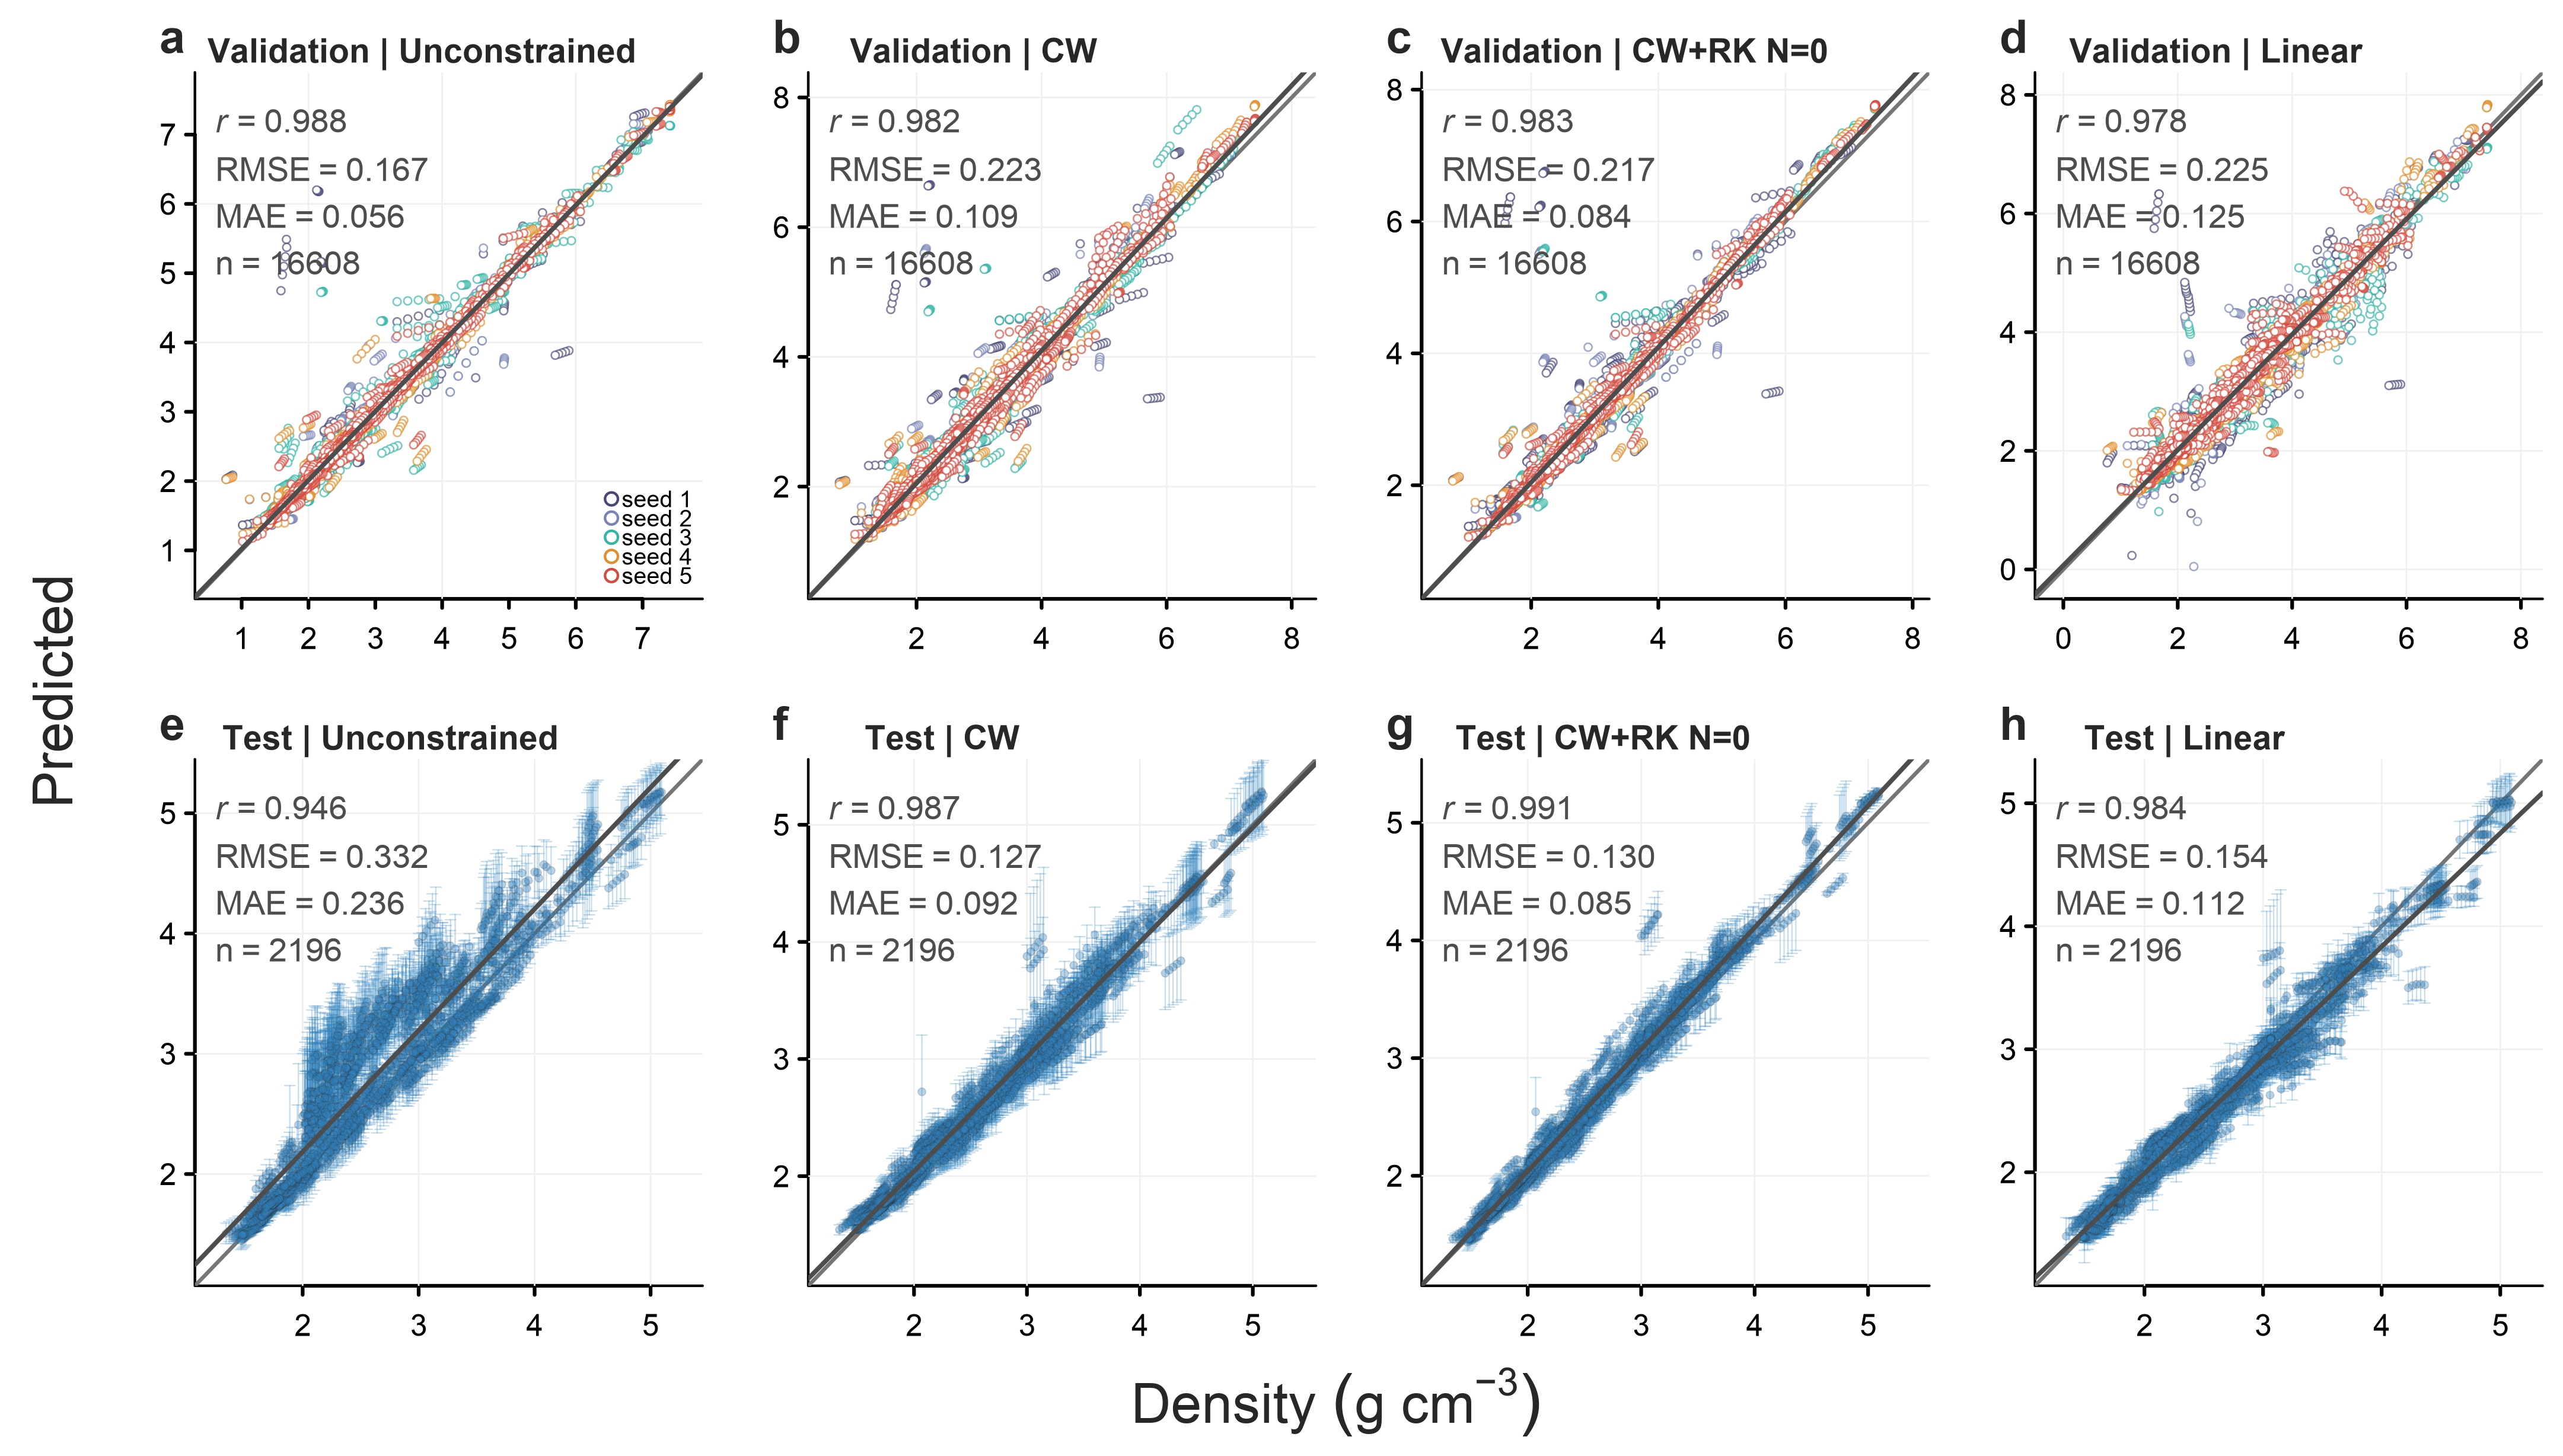
\includegraphics[width=\linewidth]{density_correlation_grid.png}
      }{%
        \figmissing{Density correlation grid}
      }
      \slidecaption{Figure 3: Density prediction-reference correlations.}
    \end{column}
    \begin{column}{0.38\textwidth}
      \footnotesize
      \begin{itemize}
        \item Test systems favor \best{CW+RK with $N=0$}.
        \item Test RMSE and MAE reach $0.14\pm0.01$ and $0.10\pm0.01$.
        \item Higher RK orders do not improve extrapolation.
      \end{itemize}
      \vspace{0.10cm}
      \best{Takeaway:} Density behaves like a bulk non-ideal mixing problem where low-order pair corrections are useful.
    \end{column}
  \end{columns}
\end{frame}

\begin{frame}{Surface Tension: Metric-Dependent Ranking}
  \begin{columns}[T,onlytextwidth]
    \begin{column}{0.57\textwidth}
      \IfFileExists{../saltmix-manuscript/figures/surface_tension_correlation_grid.png}{%
        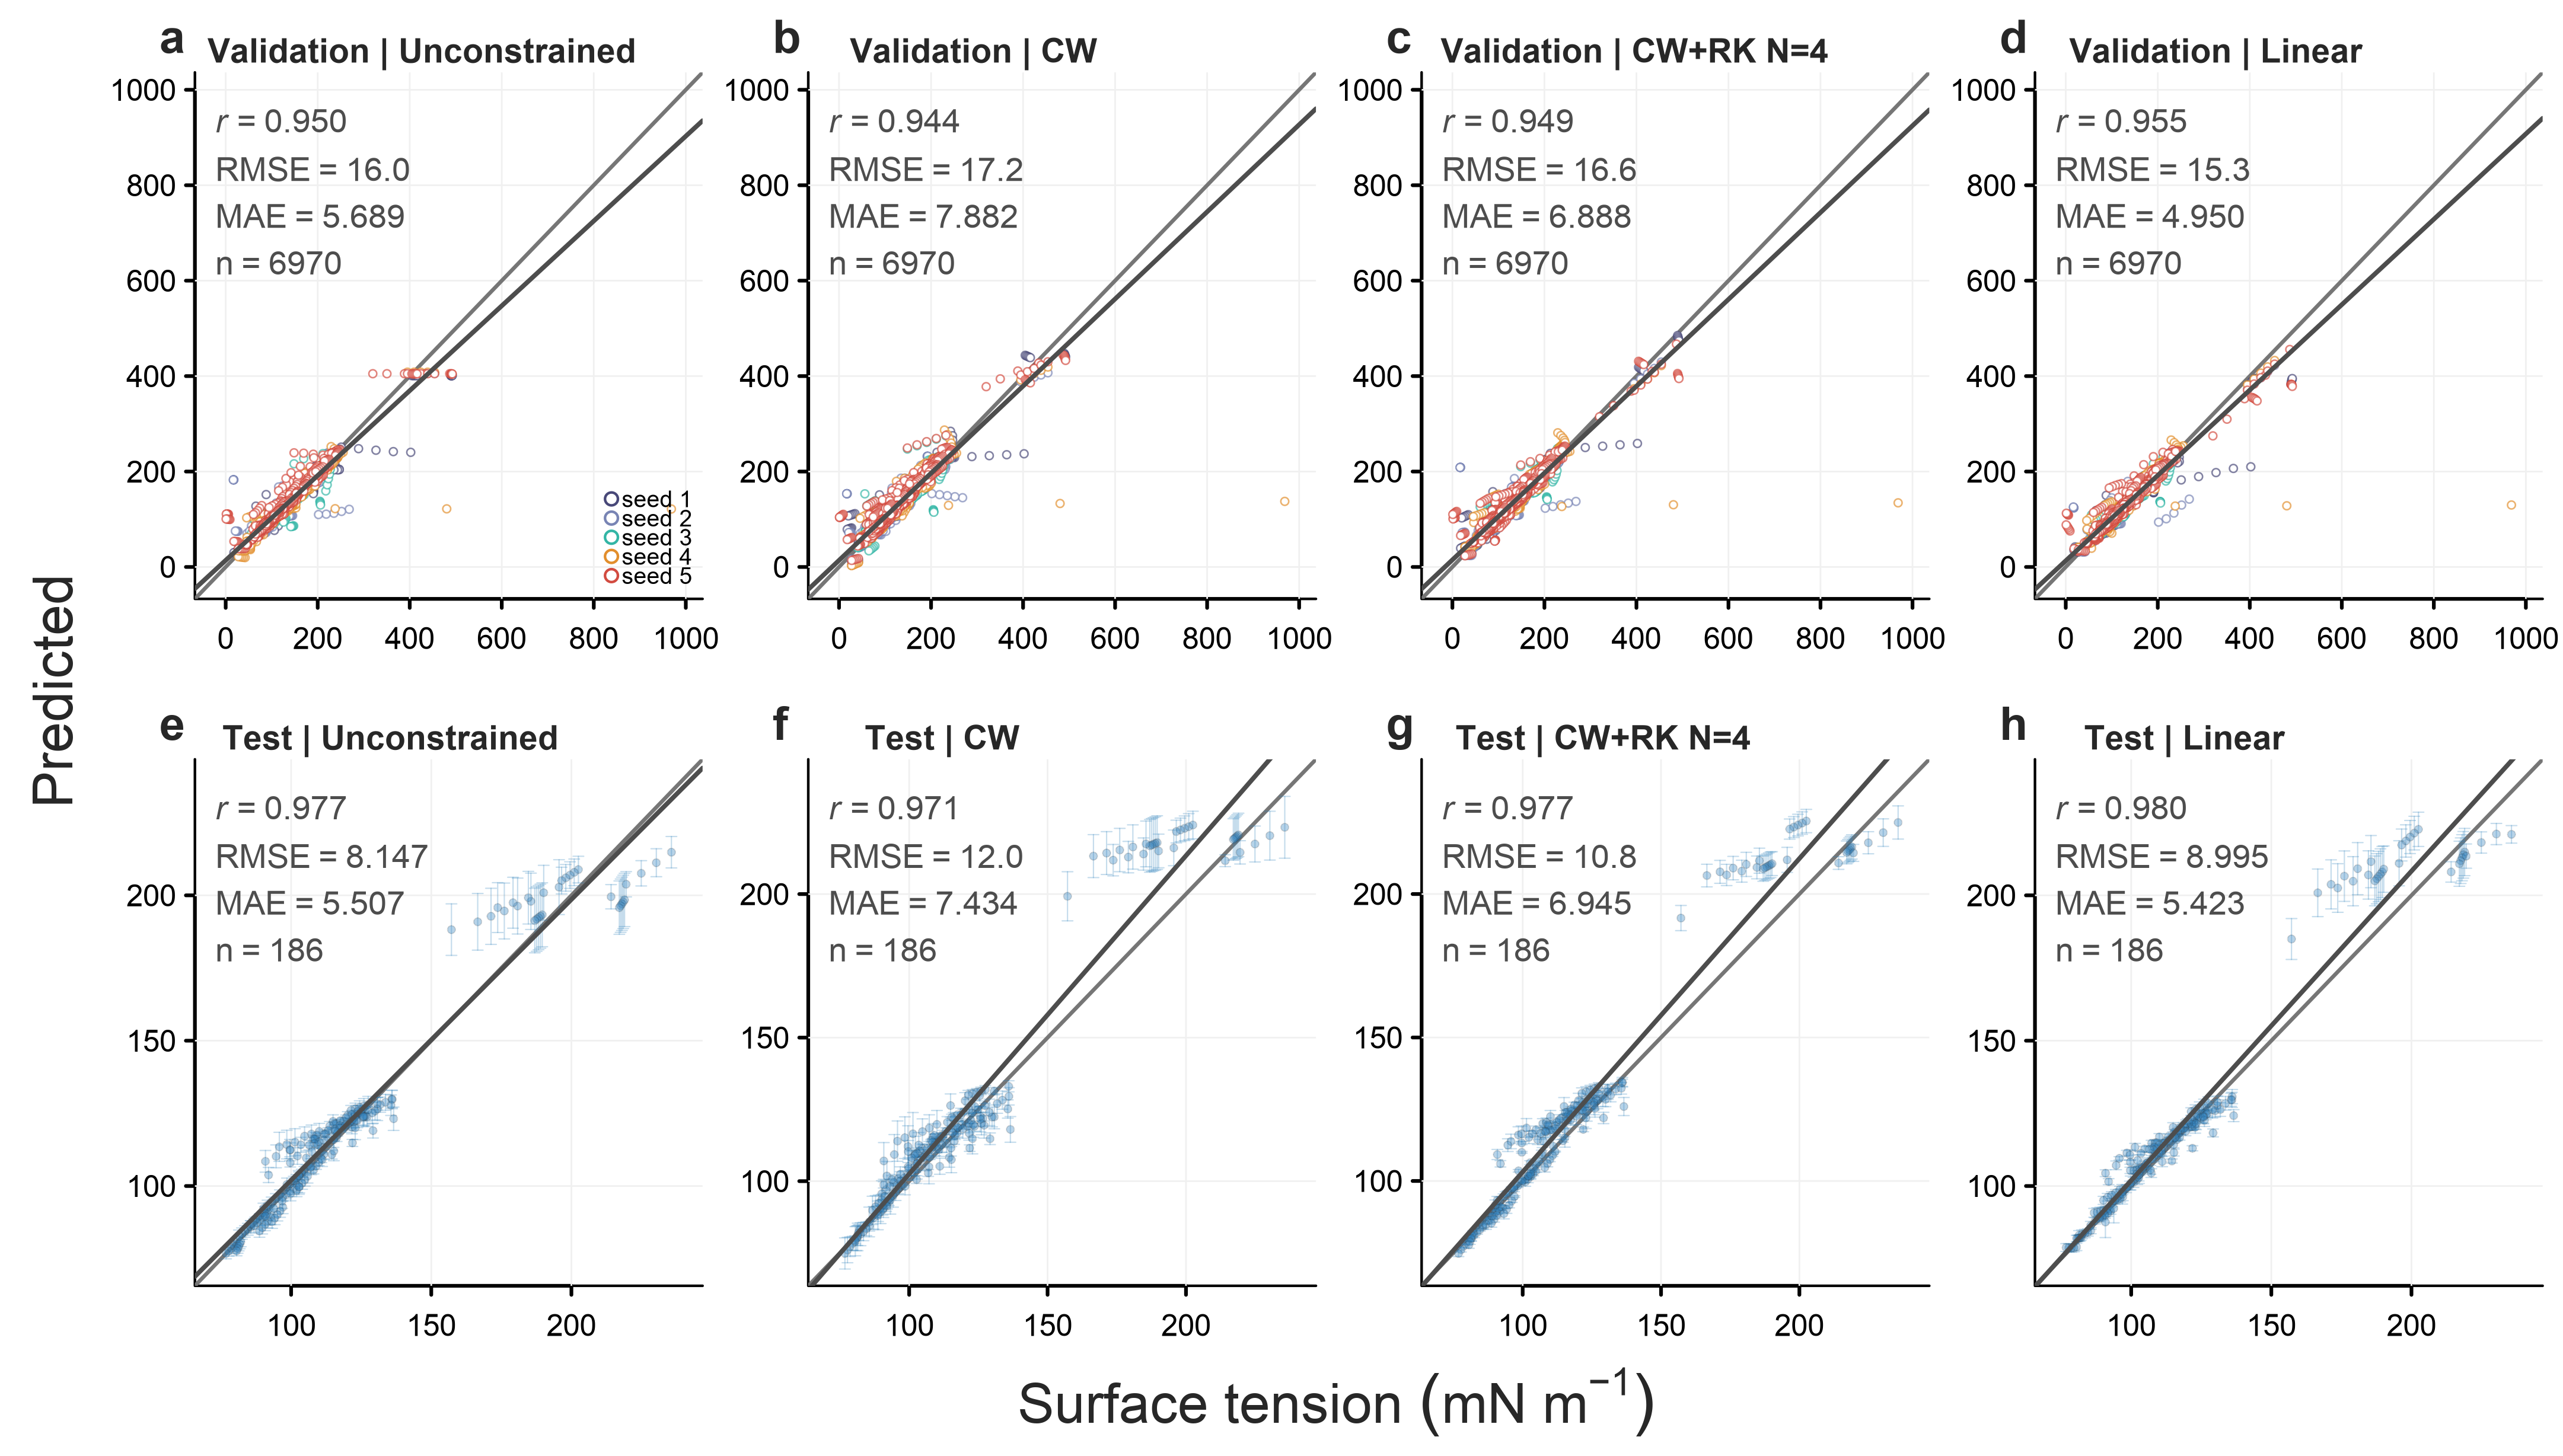
\includegraphics[width=\linewidth]{surface_tension_correlation_grid.png}
      }{%
        \figmissing{Surface-tension correlation grid}
      }
      \slidecaption{Figure 4: Surface-tension prediction-reference correlations.}
    \end{column}
    \begin{column}{0.38\textwidth}
      \footnotesize
      \begin{itemize}
        \item Linear model gives the best validation performance.
        \item Test RMSE is lowest for unconstrained: $8.75\pm1.80$.
        \item Test MAE and $r$ are best for linear: $5.66\pm0.88$ and $0.98\pm0.00$.
        \item CW+RK variants show no consistent advantage.
      \end{itemize}
      \vspace{0.10cm}
      \best{Takeaway:} Interfacial behavior is not directly encoded by bulk pairwise RK terms.
    \end{column}
  \end{columns}
\end{frame}

\begin{frame}{Viscosity: Arrhenius Constraint Transfers Best}
  \begin{columns}[T,onlytextwidth]
    \begin{column}{0.57\textwidth}
      \IfFileExists{../saltmix-manuscript/figures/viscosity_correlation_grid.png}{%
        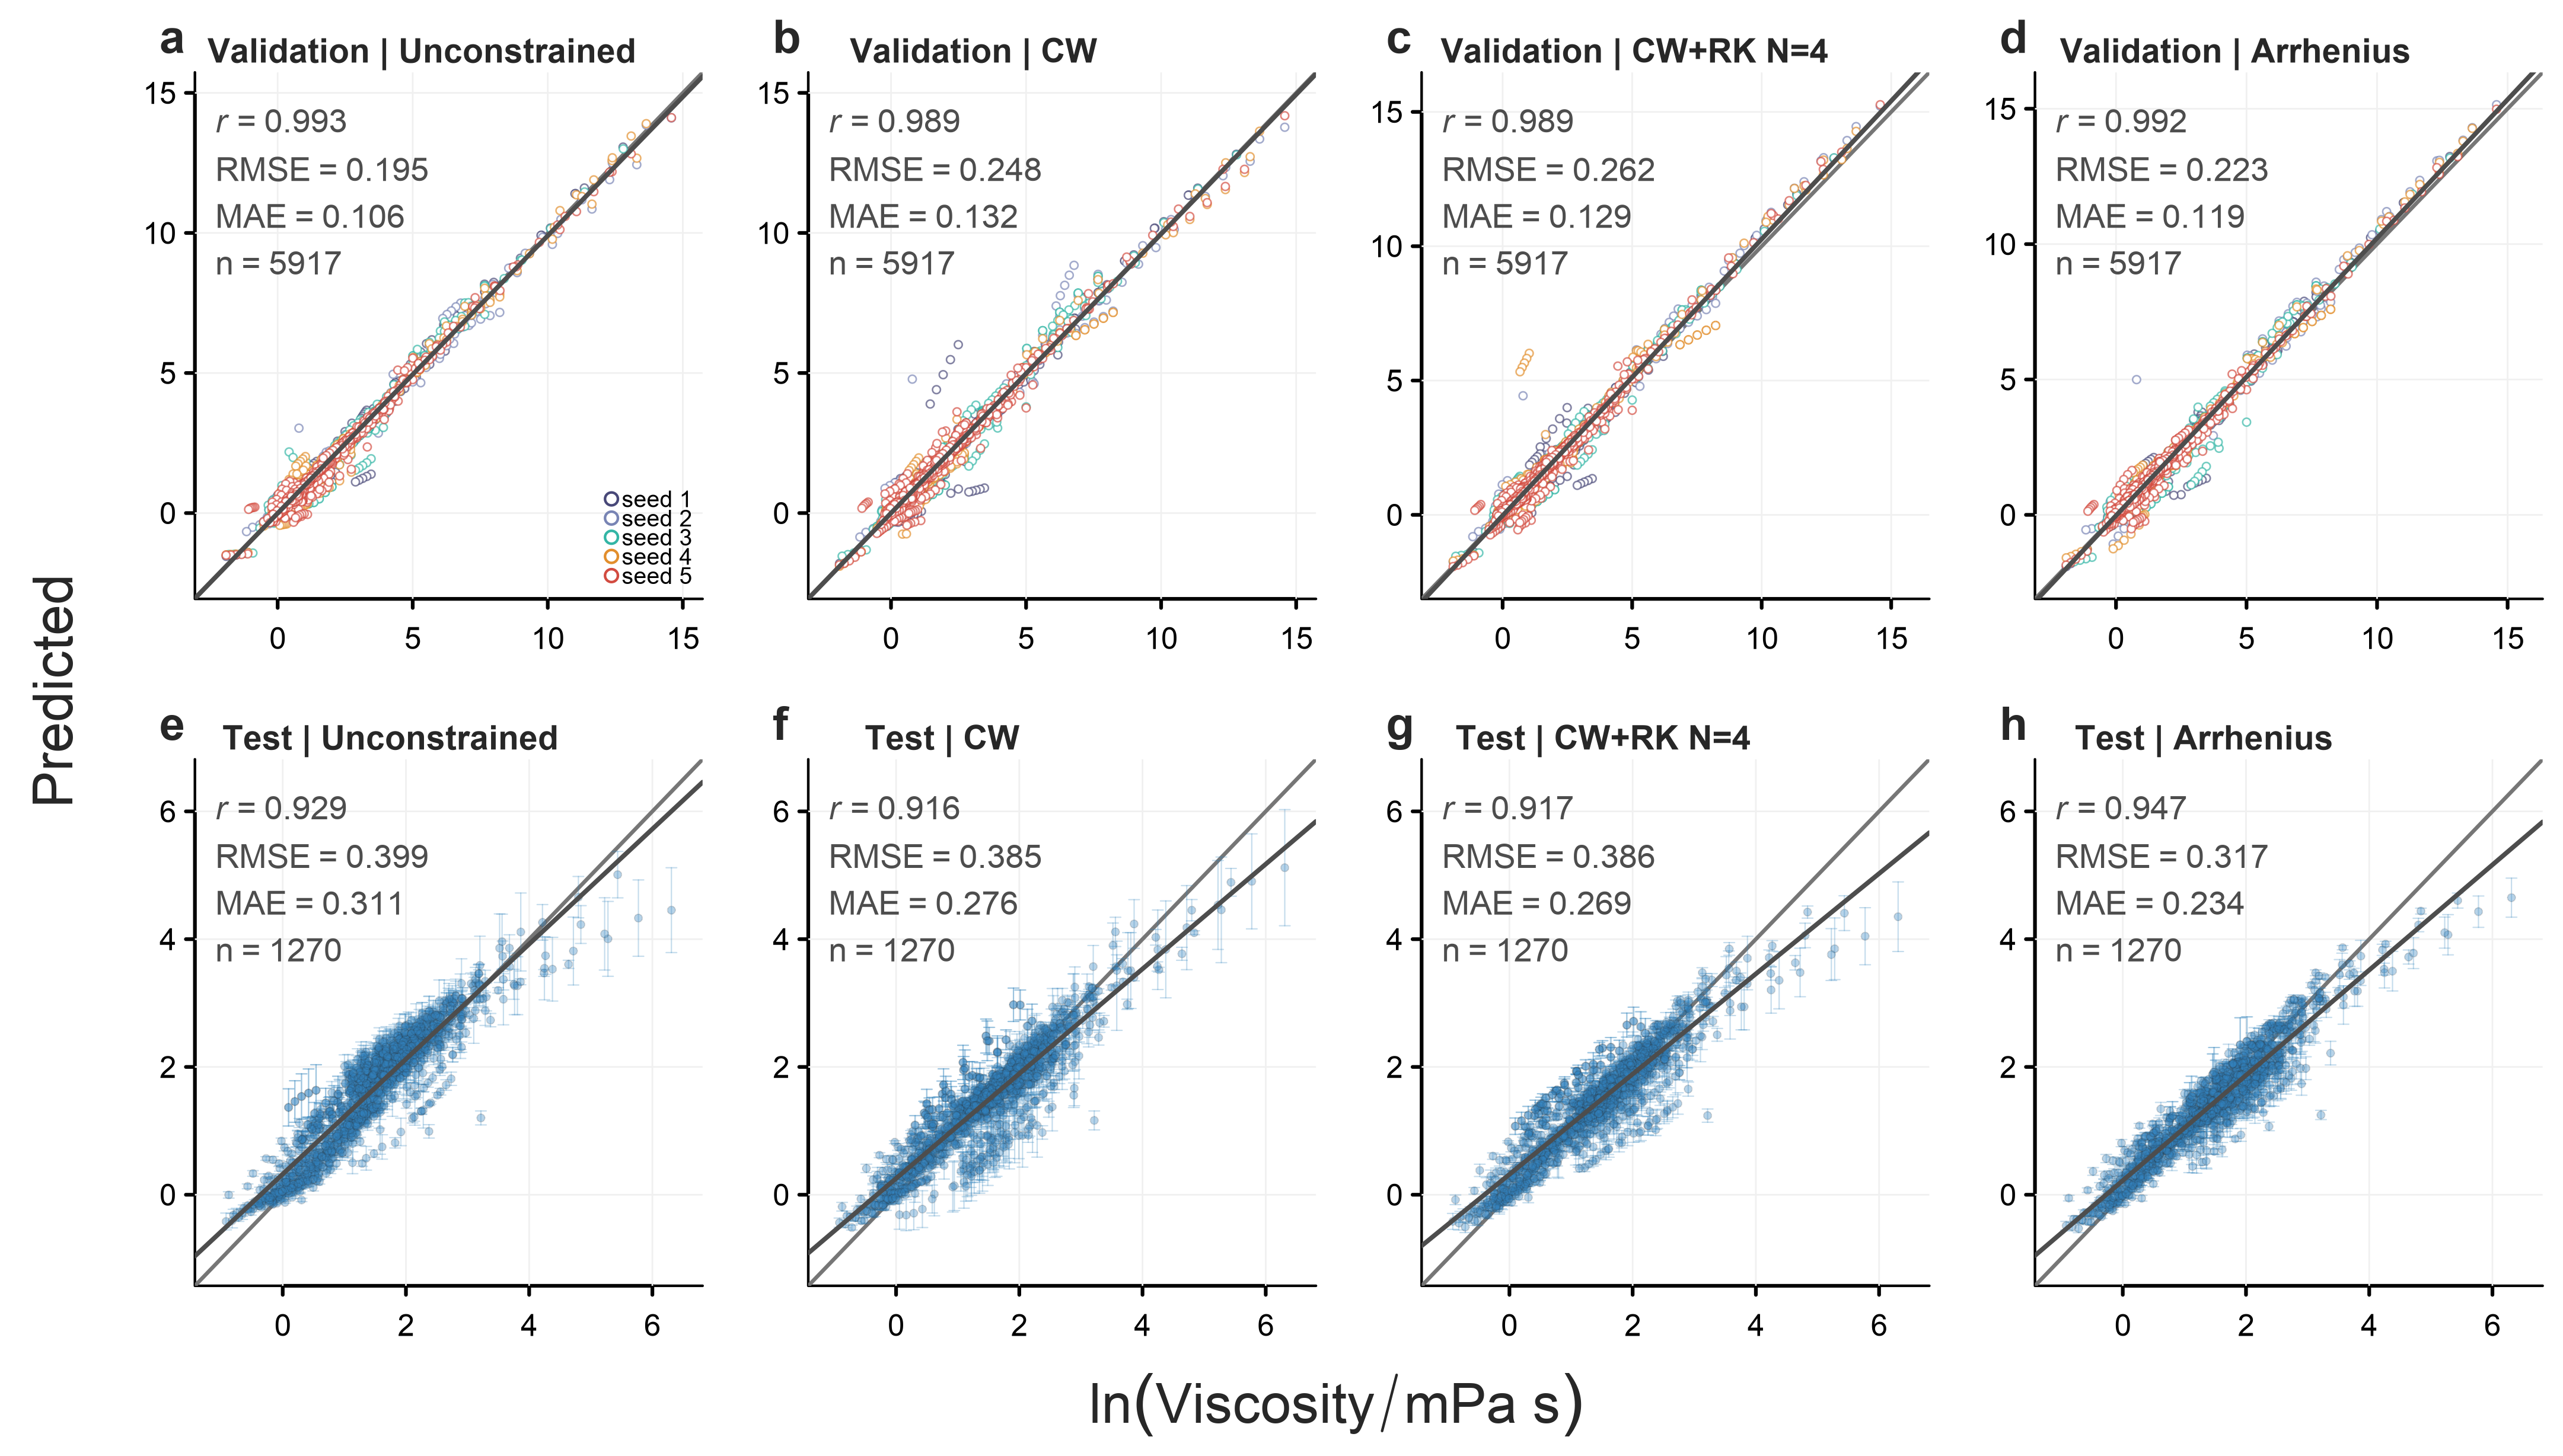
\includegraphics[width=\linewidth]{viscosity_correlation_grid.png}
      }{%
        \figmissing{Viscosity correlation grid}
      }
      \slidecaption{Figure 5: Viscosity prediction-reference correlations.}
    \end{column}
    \begin{column}{0.38\textwidth}
      \footnotesize
      \begin{itemize}
        \item Test performance is best for the \best{Arrhenius} model.
        \item Test RMSE, MAE, and $r$: $0.33\pm0.04$, $0.25\pm0.03$, $0.94\pm0.02$.
        \item CW+RK order increases do not close the gap.
      \end{itemize}
      \vspace{0.10cm}
      \best{Takeaway:} Viscosity is controlled by thermally activated structural relaxation and flow.
    \end{column}
  \end{columns}
\end{frame}

\begin{frame}{Electrical Conductivity: Flexible Plus Activated}
  \begin{columns}[T,onlytextwidth]
    \begin{column}{0.57\textwidth}
      \IfFileExists{../saltmix-manuscript/figures/electrical_conductivity_correlation_grid.png}{%
        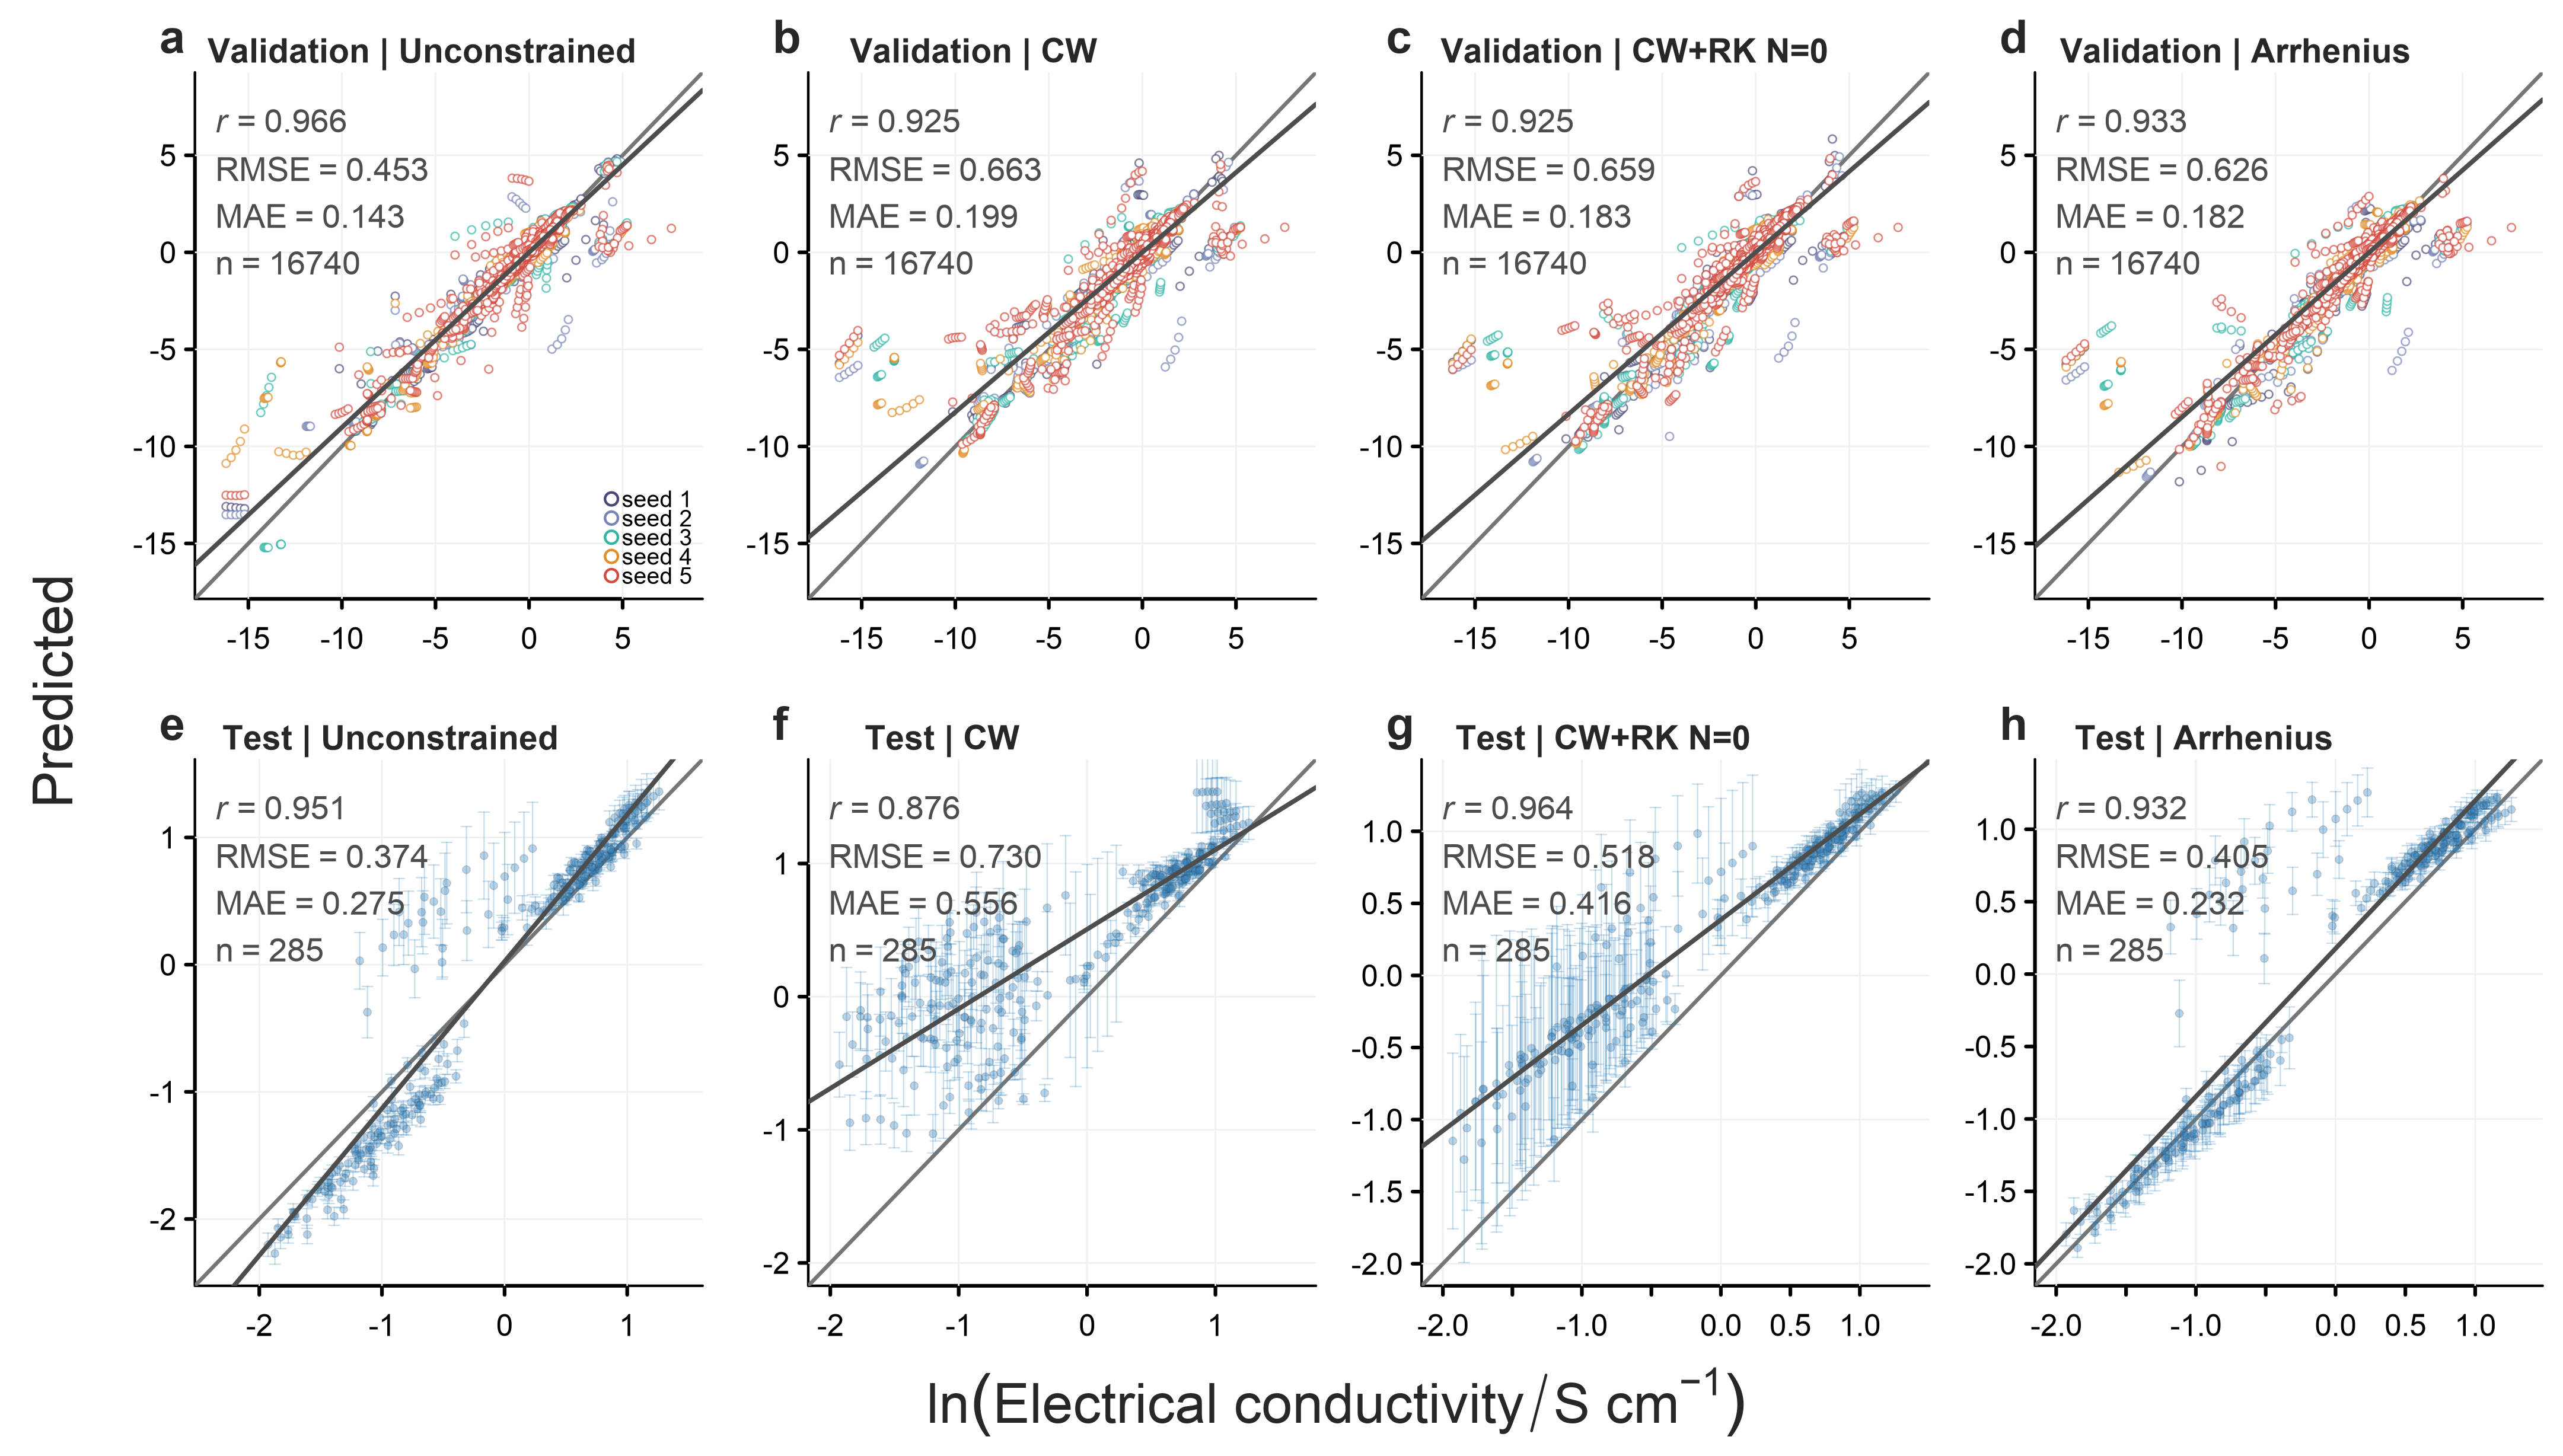
\includegraphics[width=\linewidth]{electrical_conductivity_correlation_grid.png}
      }{%
        \figmissing{Electrical-conductivity correlation grid}
      }
      \slidecaption{Figure 6: Electrical-conductivity prediction-reference correlations.}
    \end{column}
    \begin{column}{0.38\textwidth}
      \footnotesize
      \begin{itemize}
        \item Unconstrained is best by test RMSE and $r$: $0.38\pm0.07$, $0.95\pm0.02$.
        \item Arrhenius is best by MAE: $0.25\pm0.03$.
        \item Higher RK order reduces test performance.
      \end{itemize}
      \vspace{0.10cm}
      \best{Takeaway:} Conductivity needs temperature dependence plus composition flexibility.
    \end{column}
  \end{columns}
\end{frame}

\section{Discussion}

\begin{frame}{Property-Matched Inductive Biases}
  \begin{columns}[T,onlytextwidth]
    \begin{column}{0.48\textwidth}
      \begin{block}{Bulk mixing}
        \textbf{Density:} low-order RK correction captures dominant pairwise non-ideality.
      \end{block}
      \begin{block}{Interfacial trend}
        \textbf{Surface tension:} linear temperature trend is stable, while RK terms miss interface-specific rearrangement.
      \end{block}
    \end{column}
    \begin{column}{0.48\textwidth}
      \begin{block}{Activated flow}
        \textbf{Viscosity:} Arrhenius form aligns with thermally activated structural relaxation.
      \end{block}
      \begin{block}{Transport with composition effects}
        \textbf{Conductivity:} activation behavior is useful, but mobility and correlated motion require flexibility.
      \end{block}
    \end{column}
  \end{columns}
  \vfill
  \centering
  \best{Use physics as a property-specific inductive bias, not as a universal constraint.}
\end{frame}

\begin{frame}{Limitations and Next Steps}
  \begin{columns}[T,onlytextwidth]
    \begin{column}{0.48\textwidth}
      \begin{block}{Current limitations}
        \begin{itemize}
          \item Data come from empirical correlations and evaluated databases.
          \item Coverage remains uneven across salt families, properties, and mixture orders.
          \item Low-order subsystem gaps drive some high-order extrapolation errors.
        \end{itemize}
      \end{block}
    \end{column}
    \begin{column}{0.48\textwidth}
      \begin{block}{Future directions}
        \begin{itemize}
          \item Extend the framework to additional properties.
          \item Explore property-specific constraints that better reflect dominant mechanisms.
          \item Evaluate model reliability using ML-accelerated simulations or independent experimental data.
        \end{itemize}
      \end{block}
    \end{column}
  \end{columns}
\end{frame}

\begin{frame}{Takeaways}
  \begin{enumerate}
    \item A component-encoded neural framework can transfer composition--temperature--property relationships from pure/binary salts to higher-order mixtures.
    \item The best extrapolation model is property dependent: RK for density, linear/unconstrained for surface tension, Arrhenius for viscosity, and unconstrained/Arrhenius for conductivity.
    \item Increasing RK order does not provide a consistent extrapolation gain.
    \item High-order molten salt screening should choose constraints according to the target property's dominant physics.
  \end{enumerate}

  \vfill
  \begin{block}{Repository}
    Code, configurations, processed data, and selected outputs: \texttt{github.com/LiangWenshuo1118/SaltMix}
  \end{block}
\end{frame}

\end{document}
